\documentclass{../../../lessonplan}
\renewcommand{\cflroot}{../../..}

\begin{document}

\lessonplantitle
    {LKS2-S2}
    {Lower Key Stage 2 Session 2}
    {Using repeat with a condition on a simple route: repeat until}

\preamble
    {
    \item Understand how to use a conditional repeat --- \keyword{repeat until at destination}
    }
    {
    \item Levels 29 to 32 in Rapid Router
    \item Resource sheets LKS2-S2-1 to LKS2-S2-2
    \item Video 2
    \item Interactive Whiteboard (IWB)
    }
    {
    \item Repeat until
    }

\begin{lessonplan}

\fig{fig S2.1}{figS2.1.jpg}{1}

Introduce level 29 \textit{[fig S2.1]} of the app on the IWB.

Ask the children what the think \keyword{repeat until} will do.
Point out the \keyword{at destination} block.

Ask a volunteer to test this out with a simple route.

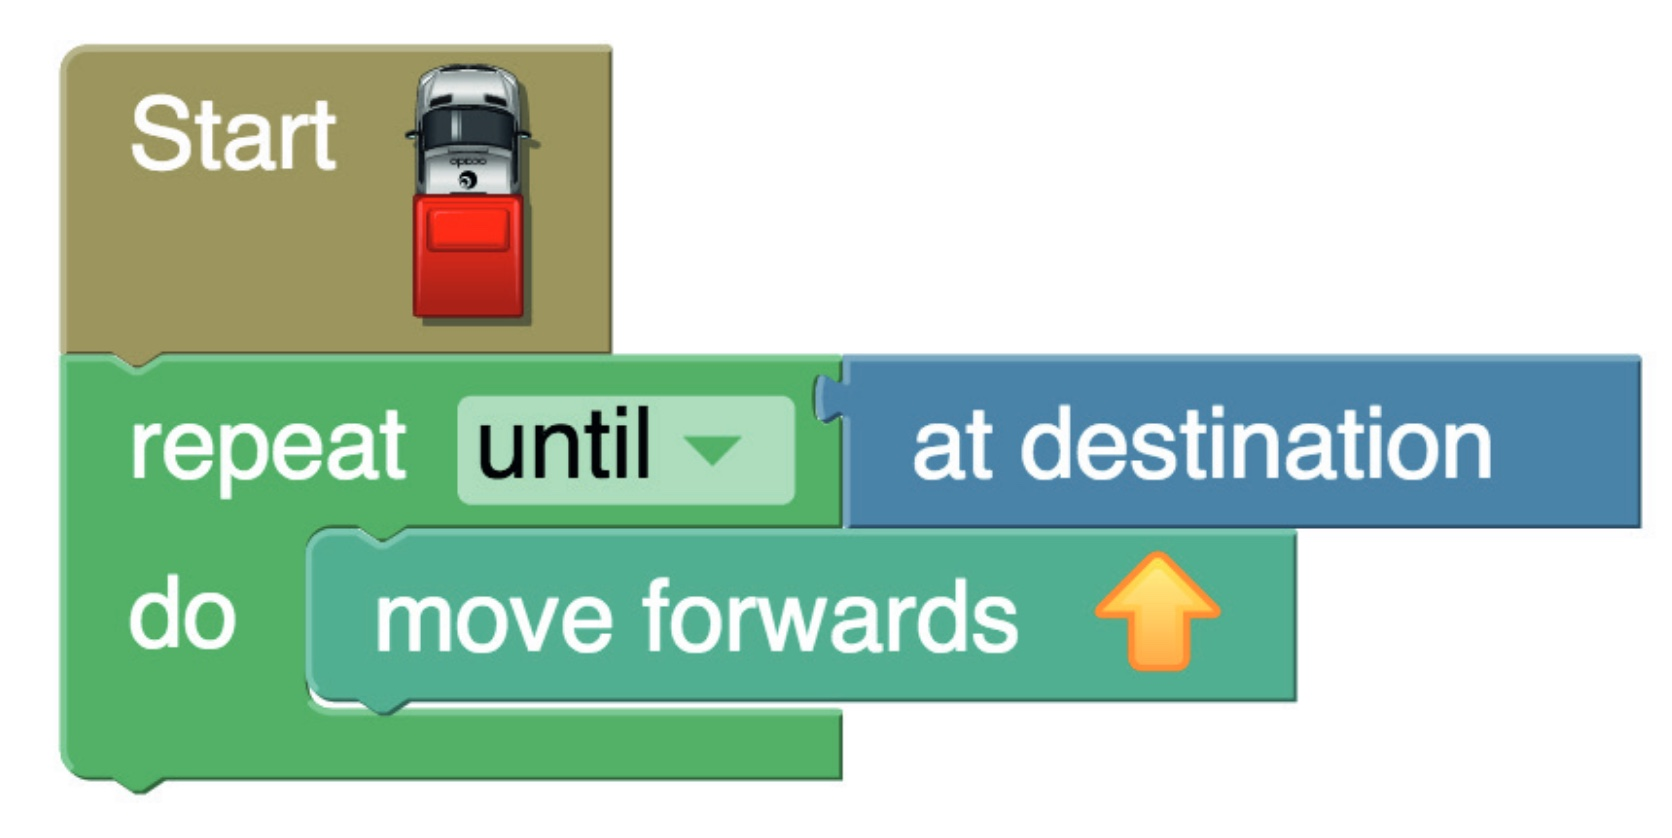
\includegraphics[width=\linewidth]{repeat_until1.jpg}

Do this again with a simple repetition of \keyword{turn left} and \keyword{turn right}.

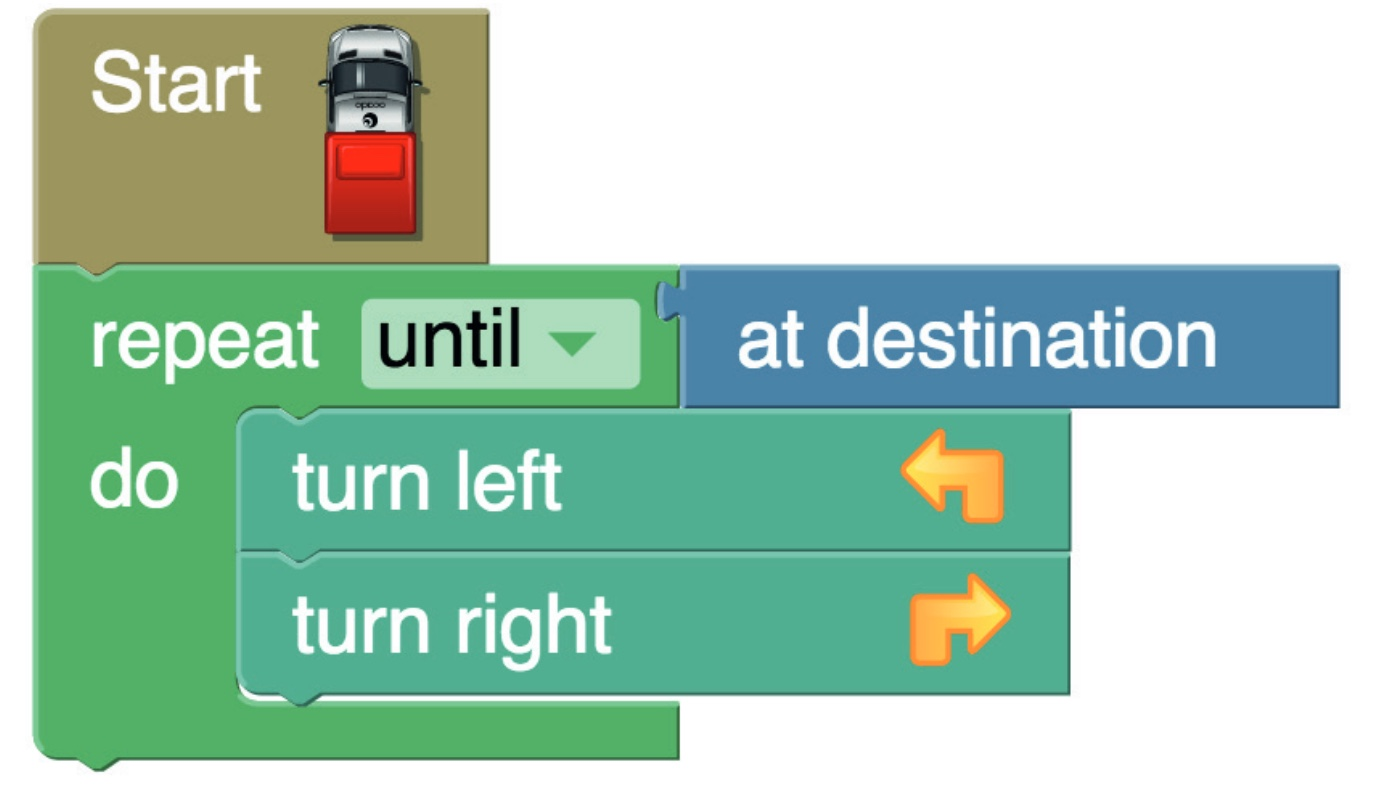
\includegraphics[width=\linewidth]{repeat_until2.jpg}

Look at \textbf{Video 2} to see Ana talking about her work and how \keyword{repeat until} is useful.

\section*{Mini review}

Ask the children to discuss with a partner the difference between using \keyword{repeat until at destination}

Set out two straight `roads' in the classroom (you can do this with masking tape, construction blocks or even by creating a route with the classroom tables) and ask two children to be van drivers at the start of each.
Ask them to `act out' the code.
\keyquestion{Will they both get to their destinations even if one route is longer? Why?}

\section*{Practical}

\fig{fig S2.2}{figS2.2.jpg}{1}

Children try out the other challenges at levels 29 to 32 \textit{[fig S2.2]}.

\section*{Share and review}

Share what has been learnt in this lesson.

\keyquestion{Can you draw two routes where \keyword{repeat until at destination (forward, left, right)} would work using LKS2-S2-1?} \textit{[fig S2.3]}.

Children discuss the unplugged activity in pairs.

Choose a pair to add the \keyword{repeat until at destination} blocks of code to your code wall, and add labels to explain what they do.

\keyquestion{Can you think of some activities which we do in the classroom, where we use \keyword{repeat until}?}

\fig{fig S2.3}{figS2.3.jpg}{1}

For example:
\begin{itemize}
  \item Filling a large container with smaller beakers of water --- `\keyword{repeat until} container is full';
  \item Playing percussion to a music track --- `\keyword{repeat until} the song is finished (tap the drum, wait 1 second)'.
\end{itemize}

\section*{Further consolidation}

Use resource sheet LKS2-S2-2 \textit{[fig S2.4]} for children to create their own \keyword{repeat until} loops.

\fig{fig S2.4}{figS2.4.jpg}{1}

\end{lessonplan}

\end{document}
